%
%	Praxisbezug
%

\pagebreak
\section{Using Rancher as an Enterprise Container Management Platform}

\onehalfspacing

\subsection{Rancher overview}

Rancher provides a solution to centrally manage multiple Kubernetes clusters in Enterprise IT, all from an user-friendly GUI

Rancher was recognized in 2019 as a Firestarter in Gartner's annual technology award program.\footnote{See \textit{Rancher Labs (2019)}: Rancher Labs Recognized by 451 Research as a ‘451 Firestarter’. \cite{firestarter451}}

The Rancher Dashboard for an active Kubernetes cluster looks like this:

\begin{figure}[h]
\centering
\caption {Rancher Dashboard}
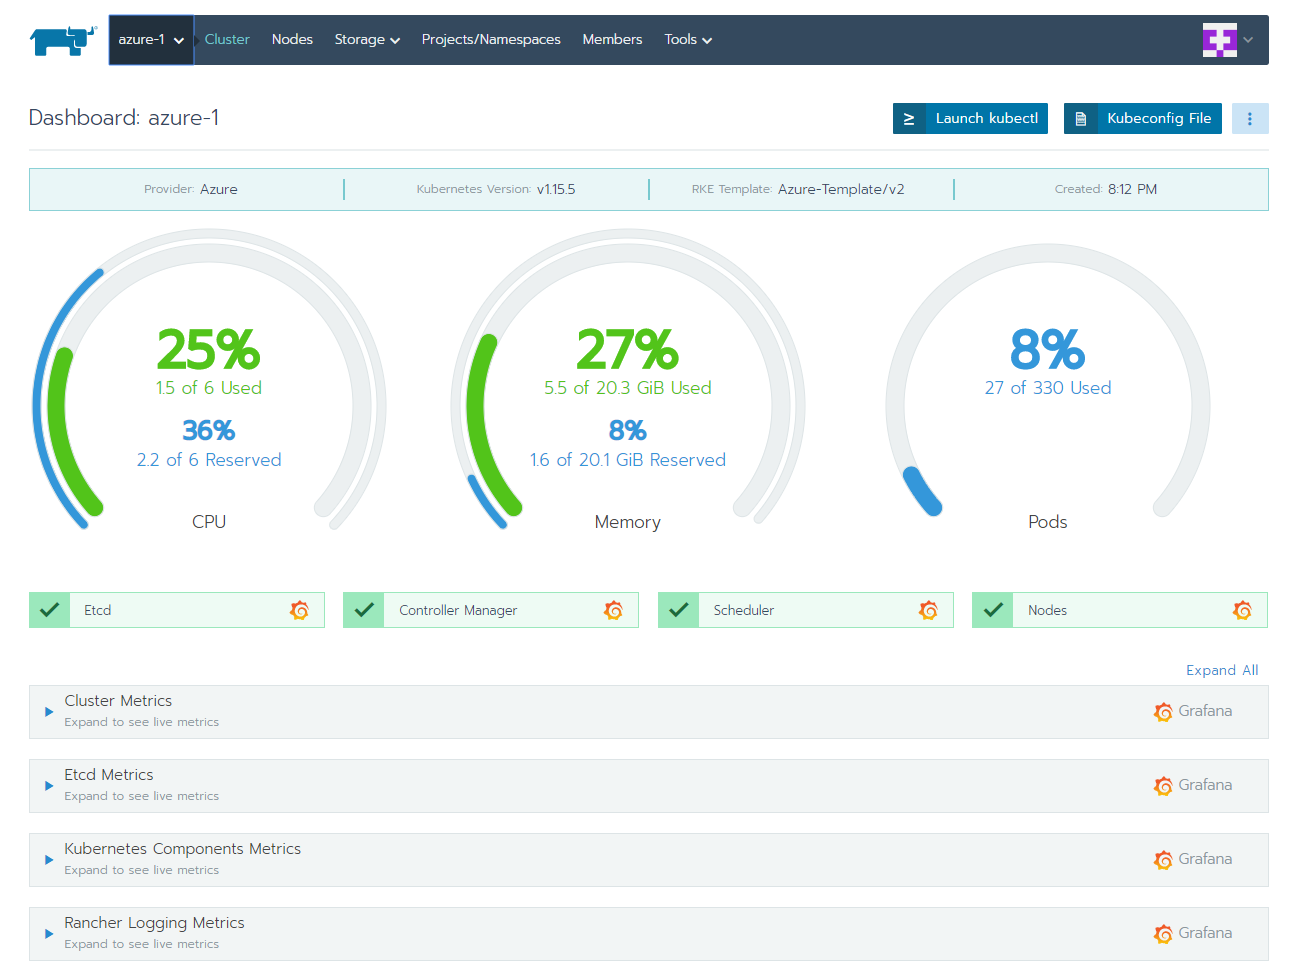
\includegraphics[width=\linewidth]{images/dashboard}
\label{fig:rancherDashboard}
\end{figure}

This cluster was created on Azure, with cluster monitoring enabled.

\subsection{User Management}

Central user authentication

Central RBAC management

\subsection{Security}

Central Policy management

Central cluster hardening\footnote{See \textit{Rancher Labs (2019)}: Hardening Guide - Rancher v2.3.x. \cite{hardeningGuide}}

Central secret management

\subsection{Cluster Management}

Central cluster management and installation

Central version control and upgrades

Central Logging and Monitoring

Automatic backup 

Cluster, Node and Credential templates

\subsection{Applications and CI/CD}

Integrated Service Mesh

Integrated pipeline

Integration with Helm

Application catalogs

Storage volumes and classes

\subsection{Infrastructure as Code}

Terraform provider\footnote{See \textit{HashiCorp (2019)}: Deliver infrastructure as code with Terraform. \cite{terraform}} \footnote{See \textit{Rancher Labs (2019)}: Introducing the Rancher 2 Terraform Provider. \cite{terraformProvider}}
